\documentclass[11pt]{article}
\usepackage{amsmath}
\usepackage{mathtools}
\usepackage{txfonts}
\usepackage[margin=1.0in]{geometry}
\usepackage{graphicx}
\usepackage{float}
\usepackage{booktabs}
\usepackage[caption=false]{subfig}
\graphicspath{ {images/} }
\usepackage{appendix}
\usepackage{url}
\usepackage{wrapfig}


\setlength{\parskip}{\baselineskip}%
\setlength{\parindent}{0pt}%
\renewcommand{\baselinestretch}{1.4}

\title{A regression model for predicting rail transit ridership at the station level}
\author{Daniel Hartig}
\date{\vspace{-5ex}}


\begin{document}
\maketitle

\section{Introduction}

The United States is undergoing a rail boom. Since 2010, new light rail lines have opened in Dallas, Los Angeles, Salt Lake City, Denver, Minneapolis, Houston, Seattle and more.  A new heavy rail line opened in Washington DC, and a commuter rail system in Orlando. As transit expands in cities in the United States, there is an opportunity to validate predictive rail ridership models. 

A survey of transit agencies \cite{Boyle2006} conducted by the Transit Cooperative Research Program showed that relatively few agencies are using quantitative models when forecasting ridership for new lines, extensions or stations under consideration for funding. Of the 35 agencies that responded to the survey, 29 use professional judgment and 28 use rules of thumb among one or more techniques used to generate ridership forecasts. Another method used by 22 agencies is service elasticity; a set of general transit demand response curves for changing transportation options, published by the Transportation Reserach Board \cite{tcrp95}. 

For quantitative methods, the most commonly used technique--by 18 of 35 surveyed agencies--is the four-step travel demand model \cite{McNally2008}, introduced by Mannheim and Florian \cite{Mannheim1979, Florian1988}. The Mannheim-Florian model's four steps are trip generation, trip distribution, mode choice and route choice. In the trip generation phase, trip endpoints are created with as production and attraction ends. In the trip distribution step, these endpoints are paired up to generate trips; for example a residence with a a job, or hotel with a tourist attraction. In the mode choice step, trips are assigned to various transportation modes, such as personal vehicle, bus, or walking. Finally, in the route choice step, a route using that mode of transportation is chosen.

An implementation of the Mannheim-Florian model can be seen in the Seattle's Sound Transit Ridership Forecasting Methodology Report \cite{ST3_2015, ST3_add}. The Sound Transit 3 (ST3) was a ballot measure that passed in 2016 for a \$54 billion expansion of the local light rail system involving 100 km of new tracks and 37 new stations. The ridership forecasting methodology report explained how the project's official ridership projections were developed. The regional area is divided into 785 Alternatives Analysis Zones and for each of these zones transit surveys and recorded ridership on local bus routes were used to complete the trip generation and trip distribution steps. The mode choice and route choice is done using an incremental logit model to predict changes in transit mode based on changes in transit mode availability.

Only seven of the 35 surveyed agencies used regression models to predict future transit ridership. This thesis proposes a regression-based model using data from the United States Census Bureau at the zip code level. The model will be trained on the zip code characteristics and ridership data from existing light and heavy rail transit systems and used to predict ridership on other rail transit systems.  

\section{Data Sources and Feature Generation}

\subsection{Data Sources for Predictor Variables}

The zip code level data for feature generation comes from the US Census Bureau and is available at \texttt{factfinder.census.gov}. There are thousands of potential data sets available. Selection of features is guided by Kuby \cite{Kuby2004}, Taylor \cite{Taylor2008}, and Currie \cite{Currie2011}, which demonstrate the significance of factors such as employment, population, universities, poverty, airports, park and ride stations, and rental units. In Yao \cite{Yao2007}, a distinction is made between `Need Index,' a series of features that depend on the characteristics around the station and are independent of the transit network, and transit network characteristics, which do depend on the transit network. To model network characteristics for each station, the sum of each characteristic for every other station within 15 and 30 minutes transit time is included as a feature of the original station. This also provides us quantitative way to express the 'centrality' dummy variable that is provided as a flag in many models \cite{Kuby2004, Durning2015}; centrality could be proportional to the count of population or jobs within 30 minutes of a station, for example.

This model emphasizes using only features that have `real' units. The only flag feature is for the presence of a park and ride parking spaces. Instead of using measures of land use mix as proposed in other models \cite{Durning2015, Gutierrez2011}, or dummy variables for universities and central business districts, the equivalent information is provided naturally as counting data in the feature set. Housing types (such as large apartment buildings versus single family homes) can stand in for land use mix, number of jobs at universities or in financial jobs can fill in for the equivalent dummy variable. A summary of the selected characteristics is provided in Appendix \ref{app:features}.

Ridership data for agencies that publish annual ridership reports is used to validate the model (see Appendix \ref{app:ridership}). Six cities were selected for this study: Boston, Chicago, Los Angeles, Atlanta, Dallas, and Denver. Several cities were eliminated from the sample set for various reasons. A limitation of the dataset is that it does not include government employment. While state level employment is significant in all potential cities, state employment levels are relatively constant from city to city. Federal employment varies greatly, however. Washington DC was eliminated due to the large impact of un-recorded federal employment. San Francisco and Philadelphia were eliminated because they have multiple rail systems without integrated fares. New York City was eliminated because it's subway has higher ridership than all other intra-urban rail systems in the country combined. 

The data closest to 2015 is used when possible to get an accurate relation between ridership and census data. The census data as well as Chicago, Dallas, and Denver's ridership statistics are from 2015. Boston's ridership is from 2014, Los Angeles' is from 2013-2014, and Atlanta's is from 2010-2013. 

We translate zip code level data into transit station specific data by sampling each zip code's geographic area to determine proximity to a transit station. For each zip code near the transit network, a set of random points within that zip code is generated using rejection sampling. For each of the those points, one or more closest stations are determined. Each point is assigned to one or more station within walking distance. Counts for the characteristics of each zip code, such as population or employment, are then assigned to each station proportional to the number of points assigned to each station.

\subsection{Rejection Sampling of Zip Code Shapefiles}

We use a Monte Carlo method to estimate feature counts near transit stations. Sample points are generated within each zip code near the transit network. Those points are assigned to whichever stations are within walking distance of the station. The ratio of points assigned to each station to total points generated for each zip code is used to assign feature counts to each station.

The US Census Bureau provides TIGER/Line shapefiles of each zip code tabulation area (ZCTA) in the United States at \url{https://www.census.gov/geo/maps-data/data/tiger-line.html}.  From a box drawn around the extremities of each zipcode's shape, random points are accepted if they are within the shapefile or rejected if they are outside it. Those points that are inside the shapefile are tested against author-created exclusion zones. These zones are shapes within the zip code's shapefile area that are known to not have any population, employment, or other countable characteristics. The exclusion zones are mostly drawn over water areas, or large parks. Those points that are inside the exclusion zones are also rejected.

The remaining points are tested for their distance to any transit stations. The area within walking distance of a station is its catchment. A standard transit catchment distance for rail is one half mile (800 m), although Guerra \cite{Guerra2012} suggests that one half mile is more appropriate for population as a feature while one quarter mile (400 m) is better for employment. A case study \cite{ElGeneidy2014} from a 2003 Montreal transit riders origin-destination survey concluded that approximately 50\% of riders of the city's urban rail transit walk less than 500 meters to their stations, while 90\% walk less than 1000 meters. The maximum walking distance is approximately 1500 meters. Another analysis \cite{Gutierrez2011} found the optimal distance for  for assigning population and employment to a station was between 600 and 900 meters in straight line distance.

Given this information, we choose cutoffs of 500 meters and 1000 meters for calculating station distances. Each tested point is divided between all stations within 500 meters. If there are no stations within 500 meters, then the point is divided between all stations within 1000 meters. If no stations are within 1000 meters, that point is not assigned to any station. The total sum of points and fractional points assigned to each station is divided by the total points available. The station's portion of each of the zip code's characteristic data counts is assigned to that transit station. 

\begin{figure}
\begin{center}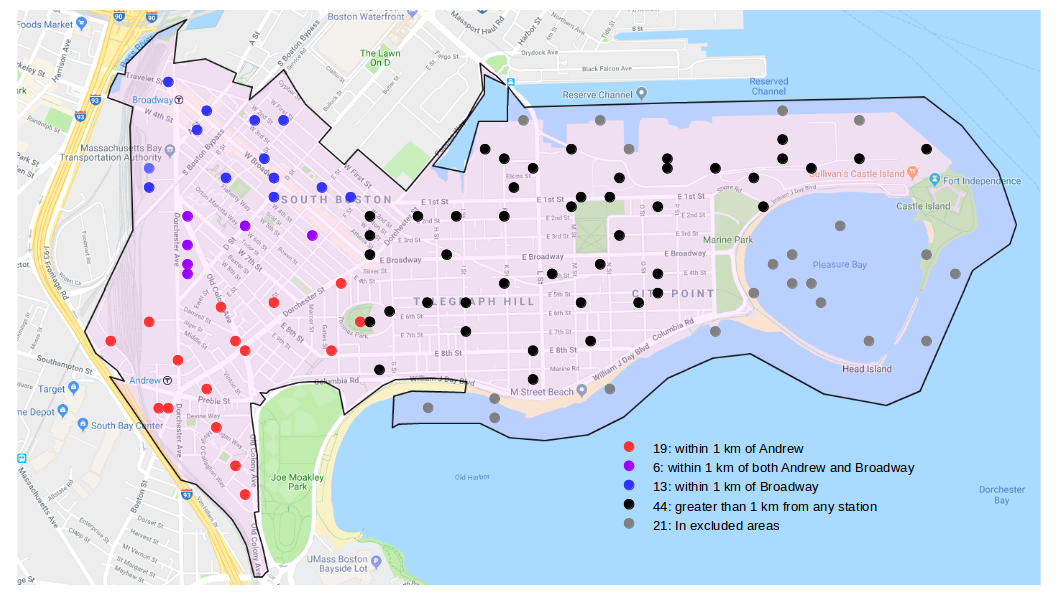
\includegraphics[scale=0.55]{geo_point_demonstration}\end{center}\caption{Illustration of nearest zip code estimation for zip code 02127.}\label{fig:f1}
\end{figure}


An example using zip code 02127, the South Boston neighborhood of Boston, illustrates the sampling method (Figure \ref{fig:f1}). 100 random points are selected within the area of the shapefile. Of these, 21 are rejected due to exclusion areas based on water area, parks and abandoned port facilities. Of the remaining 79 points, 8 are within 500 meters of Andrew station, while 6 are within 500 meters of Broadway station. Moving out to the 1000 meter radius, 11 are within 1 km of Andrew station, for a total of 19 closest to Andrew; 7 are within 1 km of Broadway station for a total of 13 closest to Broadway; and 6 are within 1 km of both. The 6 stations within 1 km of both stations are divided between the two. The total population of South Boston is 36494. Therefore, $$\frac{19 + \frac{6}{2}}{79}\cdot{36494} = 10163$$ people are assigned to Andrew station. Similarly, 7391 people are assigned to Broadway station. This calculation is performed for all countable features and all zip codes and summed total counts for each characteristic are used as a feature for each transit station. 

\subsection{Variance of Monte Carlo estimates}

With any Monte Carlo method, there is variance in the feature data generated. To keep variance to an acceptably low level, we must generate enough sample points in the Monte Carlo method.  The land area of the zip codes near the studied transit networks vary in size from as small as 30 hectare in downtown Chicago to as much as 18100 hectares at the suburban end of transit line in Dallas. We to provide a balance between accuracy and processing speed, we use one point per hectare, but with a minimum limit of 1000 points per zip code. This effectively provides over 10 points per hectare in for the zip codes in the densest parts of the studied networks: the downtown areas of Chicago and Boston. 

We generate 100 sets of projections for the a single feature (total population) for all stations in the six transit networks. Figure \ref{fig:mcvar} is a graph of means against standard deviation.

  

\subsection{Generation of network-dependent features}

For each `Need Index' type feature generated by rejection sampling, a set of corresponding network-based features are generated to represent the sum total of a certain characteristic (such as population or employment) within a given travel time of that station. The transit network is laid out as a graph, where nodes represent the transit stations and edges are weighted to the travel time between the stations, according to the website of the transit agency. At transfer points, there is a separate node for a single station on each line. The edge between these two nodes is the average wait time for transfer between the trains. 

\begin{figure}
\begin{center}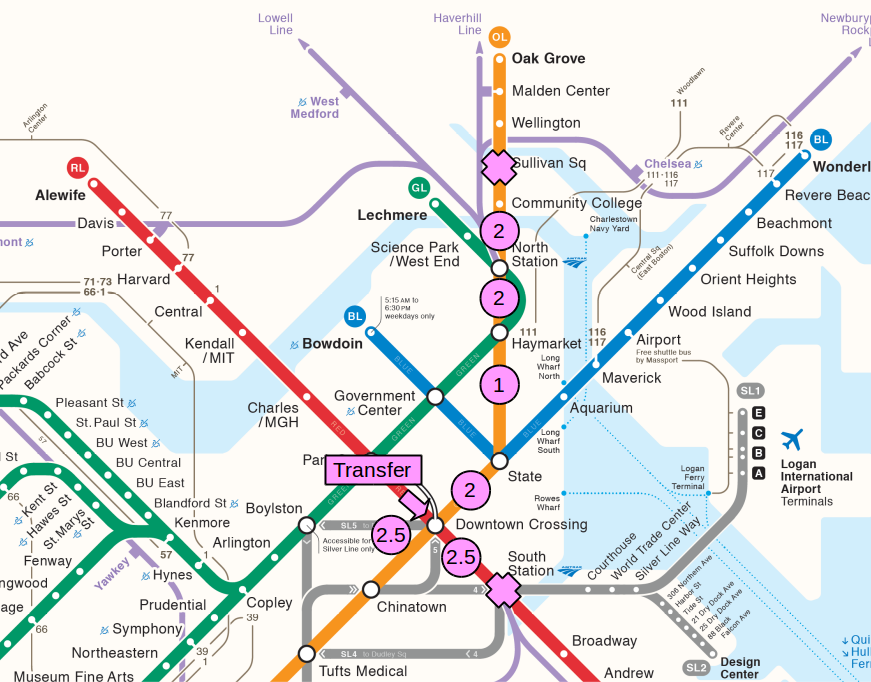
\includegraphics[scale=0.7]{transfer_demonstration}\end{center}\caption{Illustration of travel time calculation for Sullivan Square to South Station, in Boston.}\label{fig:f2}
\end{figure}

An illustration of the calculation of travel time between Sullivan Square and South Station in Boston is provided in Figure \ref{fig:f2}. Starting at Sullivan Square on the Orange Line southbound, there are four edge traversals totaling seven minutes to get to Downtown Crossing. From there, there is a 2.5 minute wait until a Red Line (also Southbound) train arrives, and 2.5 more minutes of travel to South Station. The total travel time is thus twelve minutes. 

For each station and each `Need Index' type feature, the total sum of all stations within 15 and 30 minutes is included as a feature of that station. These features are important for providing a measure of centrality to the network. Stations near the center of the network and at transfer points between lines will have higher counts of network features than than peripheral stations. The other important function of the network features is to provide estimates of the total scale of system ridership. The more people, jobs, and other characteristics near transit stations, the higher the overall system ridership is expected to be. This is a key component of the model's portability between different city's transit networks. 

\section{Model generation and Error Metrics}

\subsection{Metrics for assessing accuracy of predictions}

In general, the projected ridership forecasts of new transit infrastructure investments significantly overestimates transit ridership. The pioneering study in this field by Pickrell in 1989 \cite{Pickrell1989} found that for ten rail projects completed between 1977 and 1985, and assessed between 1986 and 1989, the actual ridership was between 28\% and 85\% lower than projected. A 2006 study \cite{Flyvbjerg2006} of 25 major passenger rail projects in  in 14 nations found that 21 of the projects had actual ridership below projections, with the average system ridership 48\% below the projection. Accurate assessment of projection accuracy is imperative for creating ridership estimates that serve the public interest.

To assess the results of regression analysis, there should be two metrics used: one for the total system level ridership, and another for station level ridership. Following Pickrell, the metric for system-wide projection accuracy is standard percentage error in total system ridership, which we will refer to as system error. Hardy \cite{Hardy2010} extends Pickrell's analysis by including absolute station error for stations on newly added sections of an existing transit network. Following Hardy, a measure of station level error on a network is summed absolute error of all station projections. The rail networks in this study vary widely in total ridership; therefore, to allow network to network comparison, this summed absolute station error can divided by total system ridership. The resulting metric for station error given a projected ($y_{proj}$) and actual ridership ($y_{true}$) is 
$$SSE = \dfrac{\sum\limits_{i\,\in\,\text{all station}}\left|y_{proj, i} - y_{true, i}\right|}{\sum\limits_{i\,\in\,\text{all station}} y_{true, i}}$$






\begin{figure}
\centering
\begin{minipage}{0.5\textwidth}
\centering
\subfloat[Ridership against population. Linear regression in red, log regression in blue.]{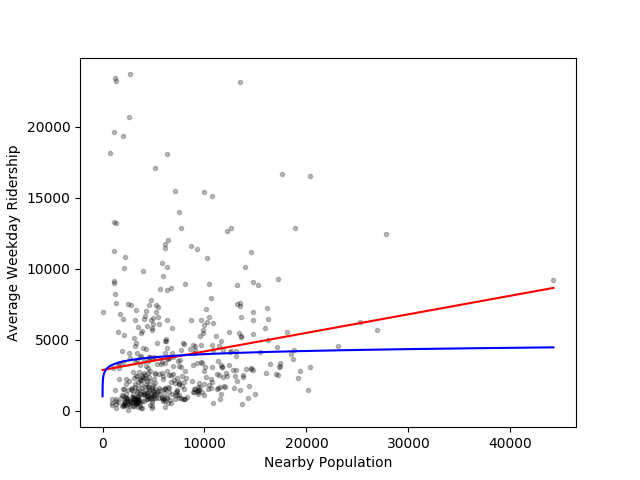
\includegraphics[clip,width=\columnwidth]{popvrider}}

\subfloat[Residual from linear regression against population]{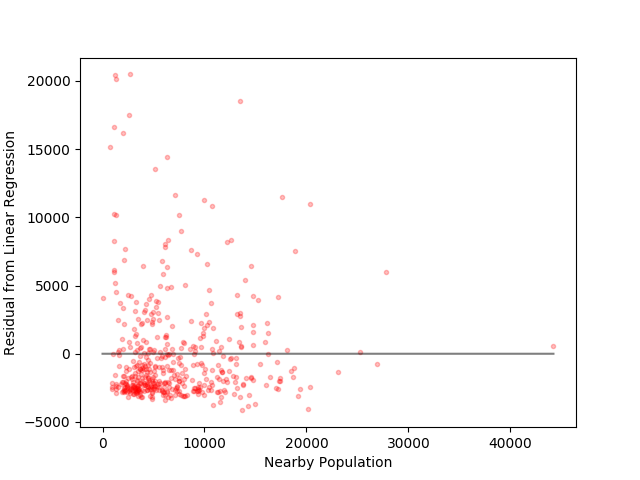
\includegraphics[clip,width=\columnwidth]{poplinresid}}

\subfloat[Residual from log regression against population]{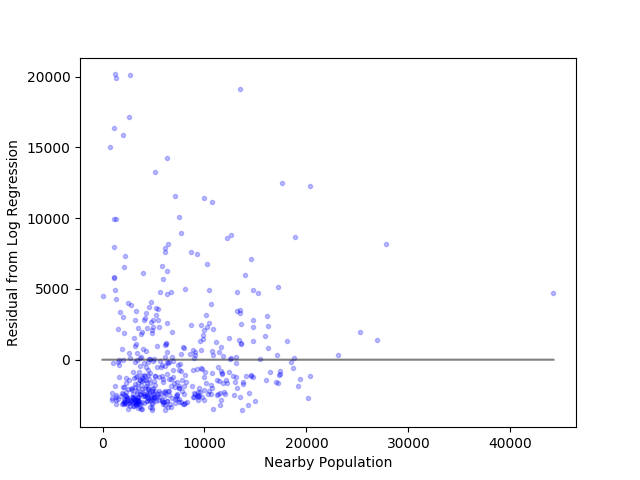
\includegraphics[clip,width=\columnwidth]{poplogresid}}
\caption{Analysis of population regression}\label{fig:popresid}
\end{minipage}\hfill
\begin{minipage}{0.5\textwidth}
\centering
\subfloat[Ridership against employment. Linear regression in red, log regression in blue.]{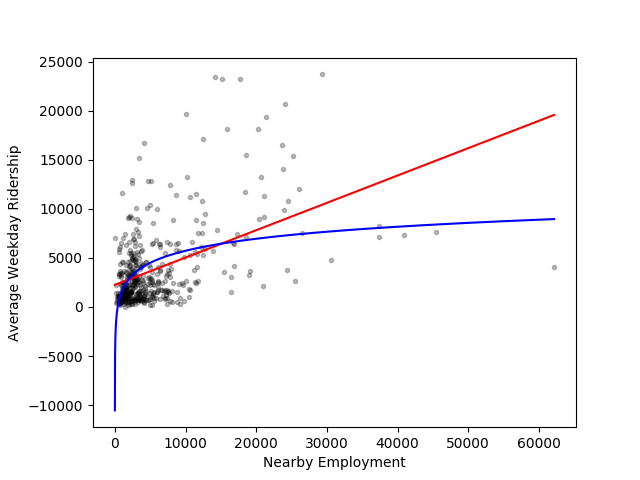
\includegraphics[clip,width=\columnwidth]{empvrider}}

\subfloat[Residual from linear regression against employment]{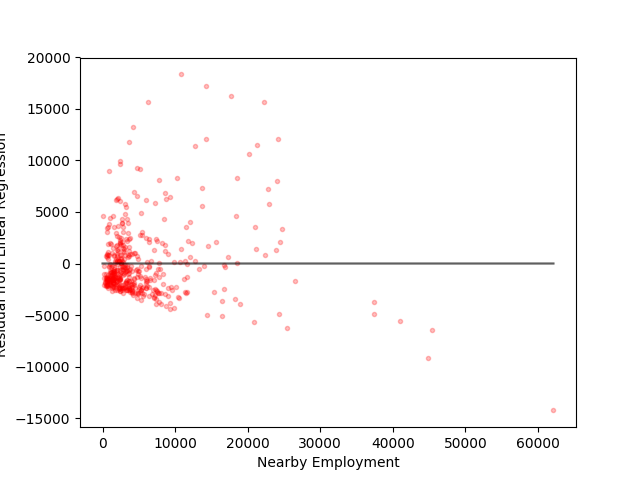
\includegraphics[clip,width=\columnwidth]{emplinresid}}

\subfloat[Residual from log regression against employment]{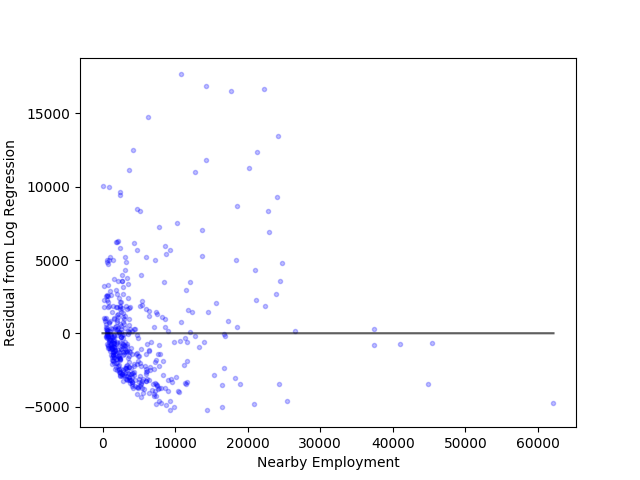
\includegraphics[clip,width=\columnwidth]{emplogresid}}
\caption{Analysis of employment regression}\label{fig:empresid}
\end{minipage}\hfill
\end{figure}


\subsection{Data distribution and regression selection}

Regression models for station level ridership have used ordinary least squares regression \cite{Kuby2004, Taylor2008, Currie2011, Durning2015, Gutierrez2011} to generate predictions. We investigate the applicability of more complex regression models.


There are generally two types of feature included in this survey: those that are related to population and those that are related to employment. Features such as the population with college degrees and number of housing units will be related to total population. Features such as the number of jobs in finance or hospitality will be related to the total number of jobs. A plot of all stations' population versus ridership appears in Figure \ref{fig:popresid} with linear and logarithmic regression lines and residuals. A similar treatment for employment versus ridership appears in Figure \ref{fig:empresid}. The coefficient of determination for the two regression types for both population and employment are shown in Table \ref{tab:regr2}.

\begin{table}
\centering
\begin{tabular}{lcc}
\toprule Variable&Linear R$^2$&Log R$^2$ \\ 
\midrule Population&0.0267&0.0034 \\
Employment&0.1948&0.1878 \\
\bottomrule
\end{tabular}
\caption{Regression of Population and Employment against ridership}\label{tab:regr2}
\end{table}

The metrics for projection accuracy depend on the absolute difference between actual and predicted ridership. This suggest that Least Absolute Deviations (LAD) regression is appropriate for this problem. Since the response variable (ridership) is counts, and the variance of ridership increases with increasing employment, we will also use Poisson regression. Finally, we will use ordinary least squares (OLS) regression as a baseline comparison, to see if the other methods have any performance advantage.

As demonstrated in Table \ref{tab:regr2}, there does not appear to be any modeling advantage from using either a linear or logarithmic link function. We are testing both version by using LAD and OLS with identity link, and Poisson with a log link.

\subsection{Feature selection by LASSO regularization}

Upon performing regression analysis, it became immediately apparent that one set of features was different from the others. The number of students within a 15 or 30 minute transit trip proved to be a very accurate measurement of system level ridership. These variable are represented in the model as \texttt{15net\_students} and \texttt{30net\_students}, respectively. We show the results of a single variable OLS regression of the one variable against ridership. The scores are the average of the six way cross-validation across the six transit networks in the study. The `best' scoring other feature (\texttt{15net\_hunits\_old}; the number of housing units built before 1940 within a 15 minute transit ride) is shown for comparison.

\begin{table}
\centering
\begin{tabular}{lcc}
\toprule Variable&System Error&Station Error\\
\midrule 30net\_students&0.1016&0.5961\\
15net\_students&0.0946&0.6197\\
15net\_hunits\_old&0.2854&0.6700\\ 
\bottomrule
\end{tabular}
\caption{Error for single variable OLS for selected features}\label{tab:students}
\end{table}

The system error scores for \texttt{30net\_students} and \texttt{15net\_students} are much lower than for any other variable, while the station error for these features are also lower than any other features. As we will see, the single-feature OLS of either of these features produces a model that is approximately as good as any other model we will develop. This raises questions about the relationship between the feature and the response variable. It is possible that the population of students within walking distance of a transit station is driven by the availability of local transit. In that case, number of students is not a valid explanatory variable. Since the relationship is unclear, but the features are outliers, we will remove all features derived from number of students from the model.

OLS and Poisson LASSO regression are performed using the \texttt{glmnet} package in R. LAD LASSO is performed using the \texttt{flare} package. The \texttt{glmnet} does automatic $\lambda$ selection; for \texttt{flare} the author created a comparable $\lambda$ search algorithm. Table \ref{tab:lasso} shows the results for the three regression types. 


\begin{table}
\centering
\begingroup\fontsize{10}{15}\selectfont
\begin{tabular}{llccccccc}
\toprule
Regression Type&Result&Boston&Chicago&Los Angeles&Atlanta&Dallas&Denver&Average\\
\midrule
OLS&System&0.3711&0.6120&0.1499&0.4218&0.5187&0.2491&0.3871\\
&Station&0.6444&0.8290&0.5077&0.5736&0.8829&0.7553&0.6988\\
&\# Features&2&7&17&10&10&10&9.3\\
\midrule
Poisson&System&0.4094&0.8617&0.0543&0.4867&0.4859&0.4416&0.4566\\
&Station&0.6470&1.0397&0.5863&0.5701&0.9137&0.9021&0.7765\\
&\# Features&5&13&26&12&27&26&18.2\\
\midrule
LAD&System&0.6161&0.8431&0.4455&0.4340&0.3347&0.2889&0.4937\\
&Station&0.6519&1.0023&0.6824&0.5809&0.7502&0.7560&0.7373\\
&\# Features&36&52&48&54&47&53&48.3\\
\end{tabular}
\caption{OLS, Poisson, and LAD LASSO regression results}\label{tab:lasso}
\endgroup
\end{table}


There is a large variance in number of features chosen, even within a single regression type. The number of features chosen varies significantly both between transit networks and between regression types. The large number of features selected by LAD LASSO regression may result from the different $\lambda$ selection methods used by the computing packages. The average of 48 features selected in this method is far too high. The transit networks have between 37 and 138 stations. Several of the LASSO selections have too many features, and some of the poor accuracy may be attributable to overfitting.



\subsection{Feature selection by brute force}



Since the data set for this problem is small--with only 466 total stations--we can validate the LASSO results using a `brute force' approach. The brute force method is a greedy search of all possible features to find the best `path' to a regression solution. First, all features are checked by regression against ridership. Since we have two 'score' metrics, we use the average of system and station error to determine the best feature in each step. Each feature is checked in six-way cross validation. Each of the six cities is used as the test set while the other five are used for the training set. The average over all six cross-validation runs for each metric is what is reported in the charts below. 


\begin{wrapfigure}{r}{0.5\textwidth}
\centering
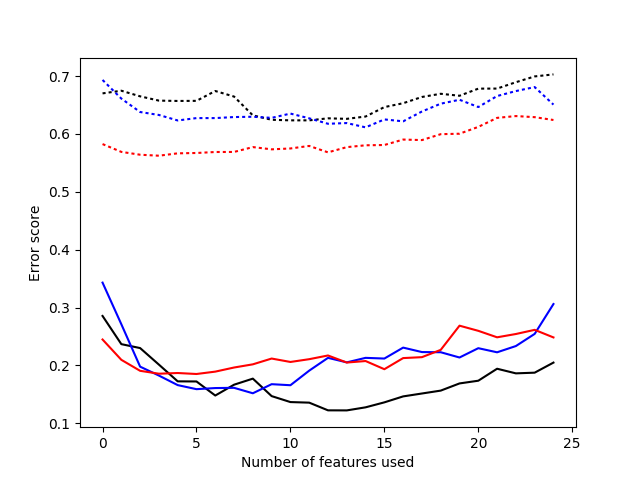
\includegraphics[width=\linewidth]{bfregress}
\vspace{-10pt}
\caption{Graph of System (solid line) and Station (dotted line) score against number of features for OLS (black), Poisson (blue), and LAD (red) regression}\label{fig:bfscores}
\end{wrapfigure}



After choosing the one feature that yields the highest score, we then select a second feature to add to the regression in in the same way, and iteratively add more features. The subsequent steps are multiple regressions using all of the already chosen features. We select the fist 25 features with this method and graph the resulting system and station error scores in Figure \ref{fig:bfscores}. 

In general, each of the error scores decreases with the addition of new variables up to a point, and then increases again. The minimum for system and station errors do not coincide with each other for any of the three regression methods, and there is a range of features which produce very similar error scores. The three regression methods each perform roughly as well as each other Error scores are averaged across the six-way cross validation. The minimum scores from each regression type are recorded in Table \ref{tab:bfresults} along with the average score over the range of good features.

The brute force regression significantly outperforms the LASSO regression in creating feature combinations that can accurately predict ridership in unknown transit networks.



\begin{table}
\begingroup\fontsize{10}{15}\selectfont
\centering
\begin{tabular}{l|ccccc}
Regression Type& Min System Err&Min Station Err& \# Features Selected& Avg System Err& Avg Station Err\\
\midrule
OLS&0.1222&0.6234&10-17&0.1342&0.6317\\
Poisson&0.1518&0.6113&4-16&0.1806&0.6255\\
LAD&0.1851&0.5623&2-16&0.1998&0.5718\\
\midrule
OLS LASSO&0.1499&0.5077&9.3&0.3871&0.6988\\
Poisson LASSO&0.0543&0.5701&18.2&0.4566&.07765\\
LAD LASSO&0.2889&0.5809&48.3&0.4937&0.7373\\
\end{tabular}
\caption{Results of brute force regression analysis, with comparison to LASSO results}\label{tab:bfresults}
\endgroup
\end{table}

A summary of selected features is given in Appendix \ref{app:featuresum}. For the brute force results, the best one feature is selected by six way cross validation for each step, from one to twenty five. Those features that fall with the range of good estimates, as shown in Table \ref{tab:bfresults}, are marked in the Appendix. 


For the LASSO feature selection, each of the six cross-validated models produces a unique set of features. Therefore, each feature is selected up to six times. We wish to avoid selection of so many features as to cause overfitting. Based on the error scores from the brute force approach, ten to fifteen features seems to be the optimal choice for all regression types. To get this number of features for each LASSO regression type, those features selected by at least four of six cross validated runs are marked in the Appendix. For the LAD LASSO, the number of features selected by LASSO is unusually high, so those features selected by at least five of size cross validated runs are selected, to avoid saturated models. 

\section{Conclusion and Future Work}

The Mannheim-Florian four step model fundamentally depends on existing transit ridership information. For example, the starting point of a four step analysis for a new light rail line would be an existing bus line that runs a similar, hopefully identical, path. The advantage of this regression model is that it creates a new estimate from different sources, independent of any knowledge of the current system.

All three regression types are able to give systemwide ridership estimates with 20\% of the true value for identified sets of between 10 and 15 features. This does not depend on any previous ridership measurement of the transit system in question and compares favorably with the 48\% average ridership prediction  error reported for 25 transportation networks in Flyvbjerg \cite{Flyvbjerg2006}. It is justifiable to use this regression based ridership model to produce and validate system-level estimates for new construction intra-urban rail transit in the United States. 

Future work in on this model could proceed in two directions. The first direction is to continue improvement of the source data. This project used only zip code shapes to estimate counting features, since job and housing data was available only for the zip code, but the population features exist in more granular detail at the Census Tract level. The author generated exclusion zones which were designed to prevent job and people from being located in parks and water could be improved by incorporating detailed city land use maps. Finally, there is a major deficiency in source data is that government workers are not included in the data sources used by the model. Of particular concern are university employment; university jobs within walking distance was a selected feature in five of the six models. Several large universities are located on the transit networks of this study and were not accounted for, such as Illinois-Chicago, Colorado-Denver, and UMass-Boston. For other cities that have very large public universities, like Minneapolis or Columbus, this would significantly affect the validity of any estimates.

The second direction is improvements of the model itself. The feature summary for this paper only analyzed selection of a feature by either the LASSO or brute force method. There remains to be done an analysis of the magnitude and direction of each feature's coefficient, to ensure that frequently selected features are significant. The R package \texttt{glmnet} is capable of performing ElasticNet regression, but for this work only $\mathcal{l}_1$, LASSO regularization was used. For OLS and Poisson, a mixed regularization may be able to improve the performance of the feature selection. 


\pagebreak
\begin{appendices}

\section{Data sources}

\subsection{Ridership data}\label{app:ridership}
\begingroup
\fontsize{9}{10}\selectfont
\begin{tabular}{ll}
Los Angeles: & \url{http://libraryarchives.metro.net/DPGTL/Ridership/RailActivityByStationFY2014.xls} \\
Chicago:& \url{http://www.transitchicago.com/assets/1/ridership_reports/2015_Annual.pdf} \\
Atlanta:& \url{http://documents.atlantaregional.com/transportation/TFB_2014_v17.pdf}\\
Boston:& \url{http://archives.lib.state.ma.us/bitstream/handle/2452/266319/ocm18709282-2014.pdf} \\
Denver:& \url{http://www.rtd-denver.com/documents/serviced/lrt-activity-08-2015.pdf} and \\
& \url{http://www.rtd-denver.com/documents/serviced/lrt-activity-Jan-April-2016.pdf}\\
Dallas:& \url{https://www.dart.org/about/dartreferencebookmar16.pdf}\\
\end{tabular}
\endgroup

\subsection{US Census feature data sources}\label{app:features}

All feature data is accessed through the American Factfinder website at \url{factfinder.census.gov}.

\begingroup
\fontsize{9}{9}\selectfont
\begin{tabular}{ll}
Population&Table DP05, Item HC01\_VC03\\
Population, 18 and under&Table DP05, Item HC01\_VC03 - Item HC01\_VC32\\
Population, 65 and over&Table DP05, Item HC01\_VC37\\
Housholds&Table S1101, Item HC01\_EST\_VC02\\
Households with Children&Table S1101, Item HC01\_EST\_VC06\\
Families&Table S1101, Item HC01\_EST\_VC010\\
Population with at least Bachelors degree&Table S1701, Item HC01\_EST\_VC34\\
Population in labor force&Table S1701, Item HC01\_EST\_VC37\\
Employed population&Table S1701, Item HC01\_EST\_VC38\\
Full-time employed population&Table S1701, Item HC01\_EST\_VC47\\
Population living at greater than 500\% of poverty level&Table S1701, Item HC01\_EST\_VC56\\
Population living at less than 200\% of poverty level&Table S1701, Item HC01\_EST\_VC01 -  HC01\_EST\_VC59\\
Housing units&Table DP04, Item HC01\_VC03\\
Single-family detached housing units&Table DP04, Item HC01\_VC14\\
Housing units in duplexes or townhouses&Table DP04, Items HC01\_VC15 + HC01\_VC16\\
Housing units in structures of 3-9&Table DP04, Item HC01\_VC17 + HC01\_VC18\\
Housing units in structures of 10+&Table DP04, Item HC01\_VC19 + HC01\_VC20\\
Housing units built before 1940&Table DP04, Item HC01\_VC36\\
Housing units built after 2000&Table DP04, Item HC01\_VC27 + HC01\_VC28 + HC01\_VC29\\
Housing units occupied by owner&Table DP04, Item HC01\_VC65\\
Housing units occupied by renter&Table DP66\\
Number of Jobs&Table CB1500CZ11, Item ‘EMP’\\
Total pay of all jobs&Table CB1500CZ11, Item ‘PAYANN’\\
Number of jobs at hospitals&Table CB1500CZ21, NAICS code 622, Estimated\\
Number of jobs at universities&Table CB1500CZ21, NAICS code 6113, Estimated\\
Number of jobs in hospitalitiy field&Table CB1500CZ21, NAICS code 72, Estimated\\
Number of jobs in finance field&Table CB1500CZ21, NAICS code 52, Estimated\\
Number of jobs in professional fields&Table CB1500CZ21, NAICS code 54, Estimated\\
Number of jobs in entertainment fields&Table CB1500CZ21, NAICS code 71, Estimated\\
\end{tabular}
\endgroup



\pagebreak
\section{Summary of selected features}\label{app:featuresum}
\hspace*{-0.4cm}
\begingroup\fontsize{9}{10}\selectfont
\begin{tabular}{llcccccc}
\toprule
&&\multicolumn{2}{c}{OLS}&\multicolumn{2}{c}{Poisson}&\multicolumn{2}{c}{LAD}\\
Variable Name&Description&LASSO&BF&LASSO&BF&LASSO&BF\\
\midrule
30net\_medical&Medical jobs within 30 min&x&x&x&x&x&\\
near\_hospitality&Hospitality jobs within walking&x&&x&x&x&x\\
near\_university&University jobs within walking&x&x&x&x&&x\\
parking&Flag for available parking&x&&x&x&x&x\\
15net\_medical&Medical jobs within 15 min&&x&&x&x&x\\
near\_business&Business jobs within walking&&x&&x&x&x\\
near\_entertainment&Entertainment jobs within walking&&x&x&x&x&\\
15net\_hunits\_attached&2-4 unit housing within 15 min&x&&x&&x&\\
15net\_hunits\_medium&5-19 unit housing within 15 min&x&&x&&x&\\
15net\_hunits\_old&Housing build before 1940 within 15 min&&x&&x&x&\\
30net\_entertainment&Entertainment jobs within 30 min&&x&&x&&x\\
30net\_hunits\_large&20+ unit housing within 30 min&&x&&x&x&\\
near\_employment&Total employment within walking&&x&x&&x&\\
near\_medical&Medical jobs within walking&&x&&x&&x\\
near\_pop\_old&Population over 65 within walking&x&&x&x&&\\
15net\_employed&Employed population within 15 min&&&&&x&x\\
15net\_hospitality&Hospitality jobs within 15 min&x&&&&x&\\
15net\_household&Housholds within 15 mins&&&&&x&x\\
15net\_university&University jobs within 15 minutes&&x&&x&&\\
near\_emp\_pay&Total employee pay within walking&&x&&&x&\\
near\_finance&Finance jobs within walking&&x&&&&x\\
near\_house\_w\_child&Households with children within walking&&x&&x&&\\
near\_hunits\_detached&Single unit housing within walking&&&&x&x&\\
near\_hunits\_owner&Owner occupied houses within walking&&&&&x&x\\
near\_hunits\_renter&Renter occupied houses within walking&&x&&x&&\\
15net\_bachelors&Population with degree within 15 min&&&&&x&\\
15net\_emp\_pay&Total employee pay within 15 minutes&&&&&x&\\
15net\_entertainment&Entertainment jobs within 15 minutes&&&&&&x\\
15net\_hunits\_renter&Renter occupied houses within 15 min&&&x&&&\\
15net\_pop\_old&Population over 65 within 15 minutes&x&&&&&\\
30net\_hospitality&Hospitality jobs within 30 min&&&x&&&\\
30net\_hunits\_medium&5-19 unit housing within 30 min&&&&&x&\\
30net\_hunits\_vacant&Vacant housing units within 30 min&&&&&x&\\
30net\_population&Total population within 30 min&&&&&&x\\
near\_emp\_full\_time&Population employed full time within walking&&&&&&x\\
near\_hunits\_attached&2-4 unit housing within walking&&&&&&x\\
near\_hunits\_large&20+ unit housing within walking&&x&&&&\\
near\_hunits\_new&Housing built after 2000 within walking&&&&&&x\\
near\_labor\_force&Population in labor force within walkin&&&&&x&\\
near\_pop\_rich&Population over 500\% of pov. level within walking&&&&&x&\\
near\_population&Total population within walking&&x&&&&\\
\end{tabular}
\endgroup
\hspace*{-0.4cm}
\end{appendices}










 
\bibliographystyle{unsrt}
\pagebreak\bibliography{bibrefs}





\end{document}